% 为了方便修改,我们可以先定义一个统一的高度变量
\newlength{\myfigheight}
\setlength{\myfigheight}{7.01cm} % 在这里统一调整三张图的高度

\begin{figure*}[t]
    \centering
    
    % --- 子图 (a) ---
    \begin{subfigure}{\widthof{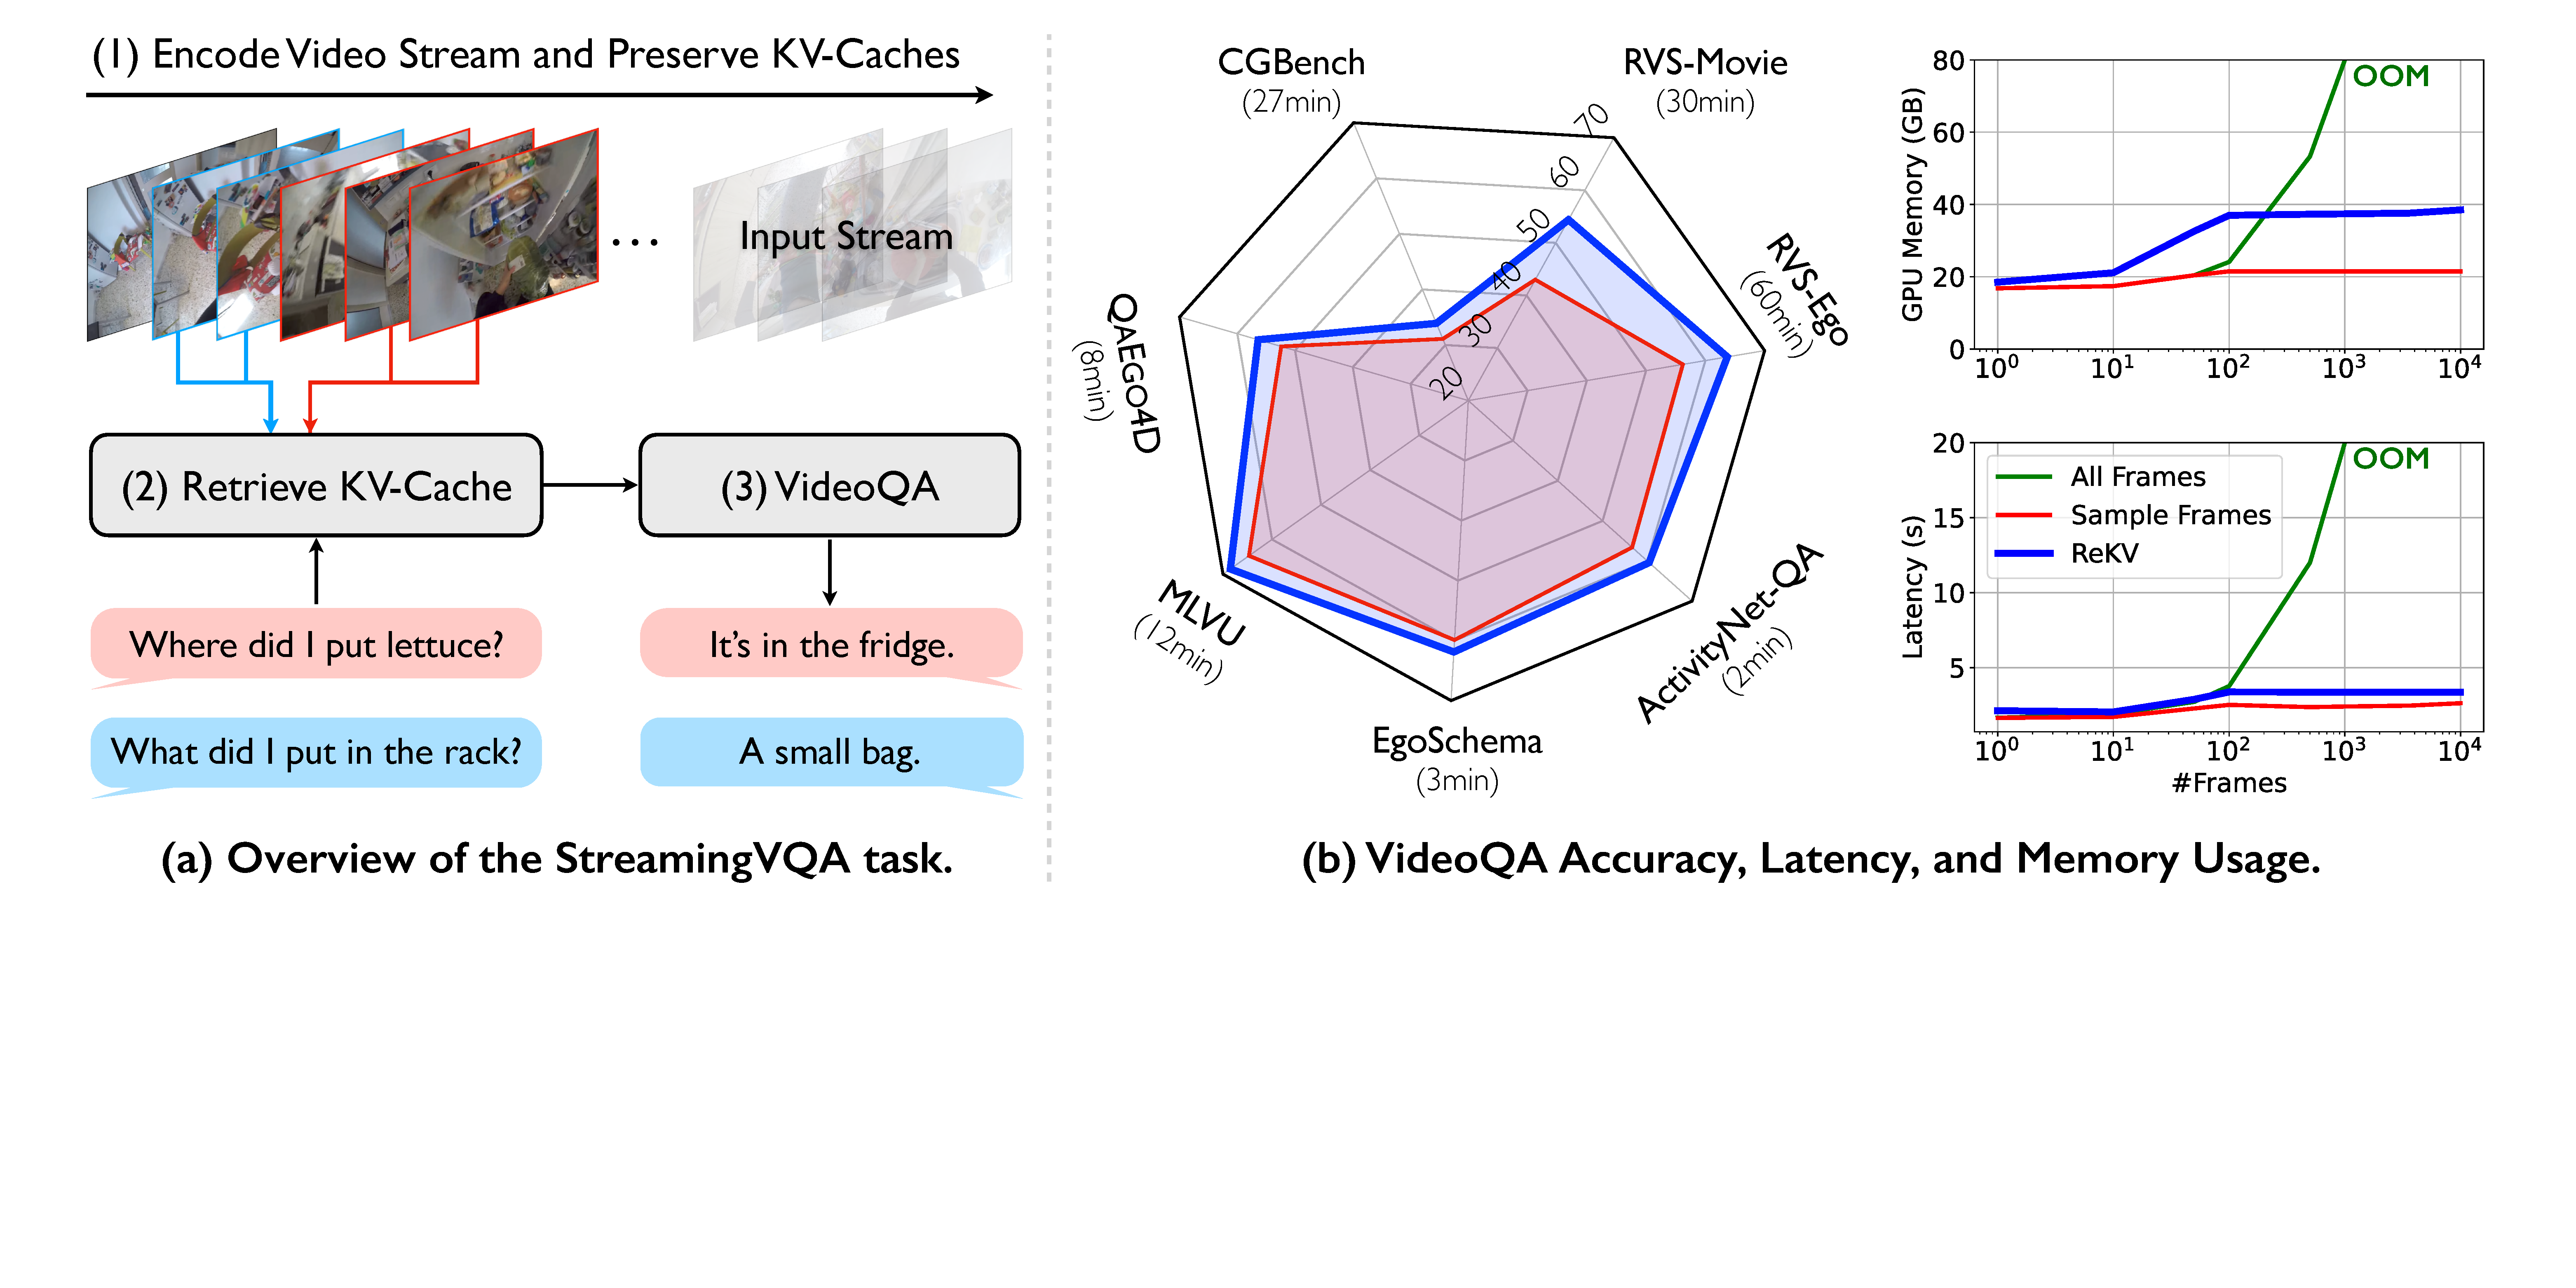
\includegraphics[height=\myfigheight, trim={0 0 415pt 0}, clip]{figures/teaser.pdf}}}
        \centering
        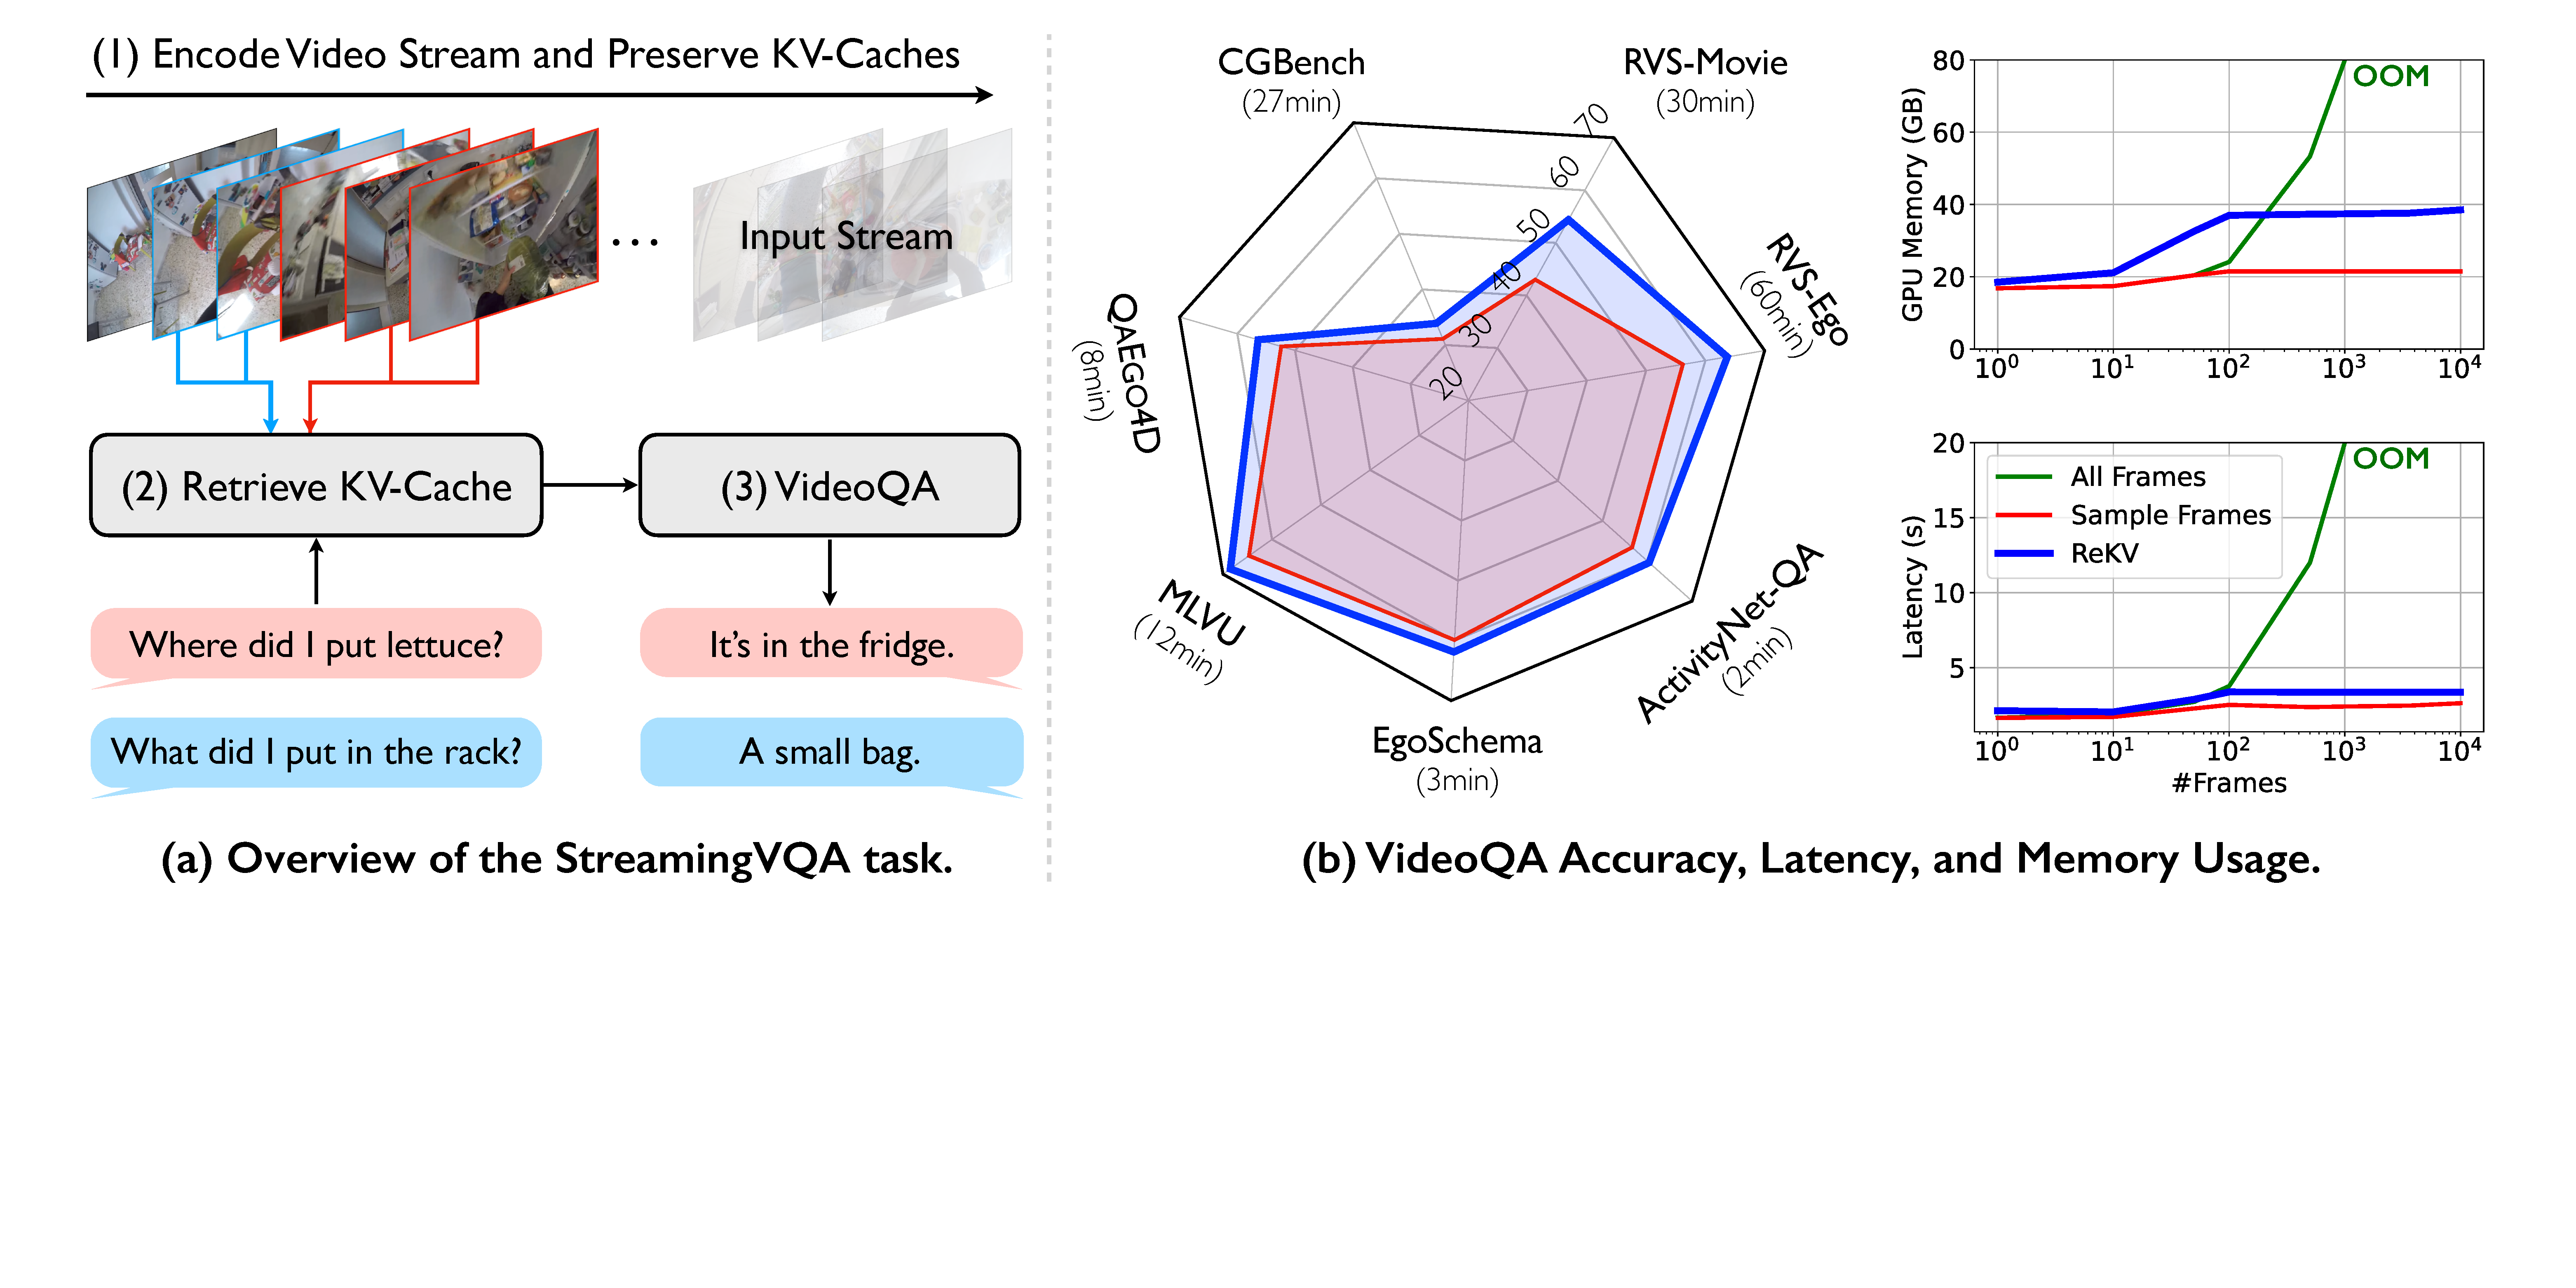
\includegraphics[height=\myfigheight, trim={0 0 415pt 0}, clip]{figures/teaser.pdf}
        \caption{\hermes Framework}
        \label{fig:teaser_a}
    \end{subfigure}
    % --- 子图 (b) ---
    \begin{subfigure}{\widthof{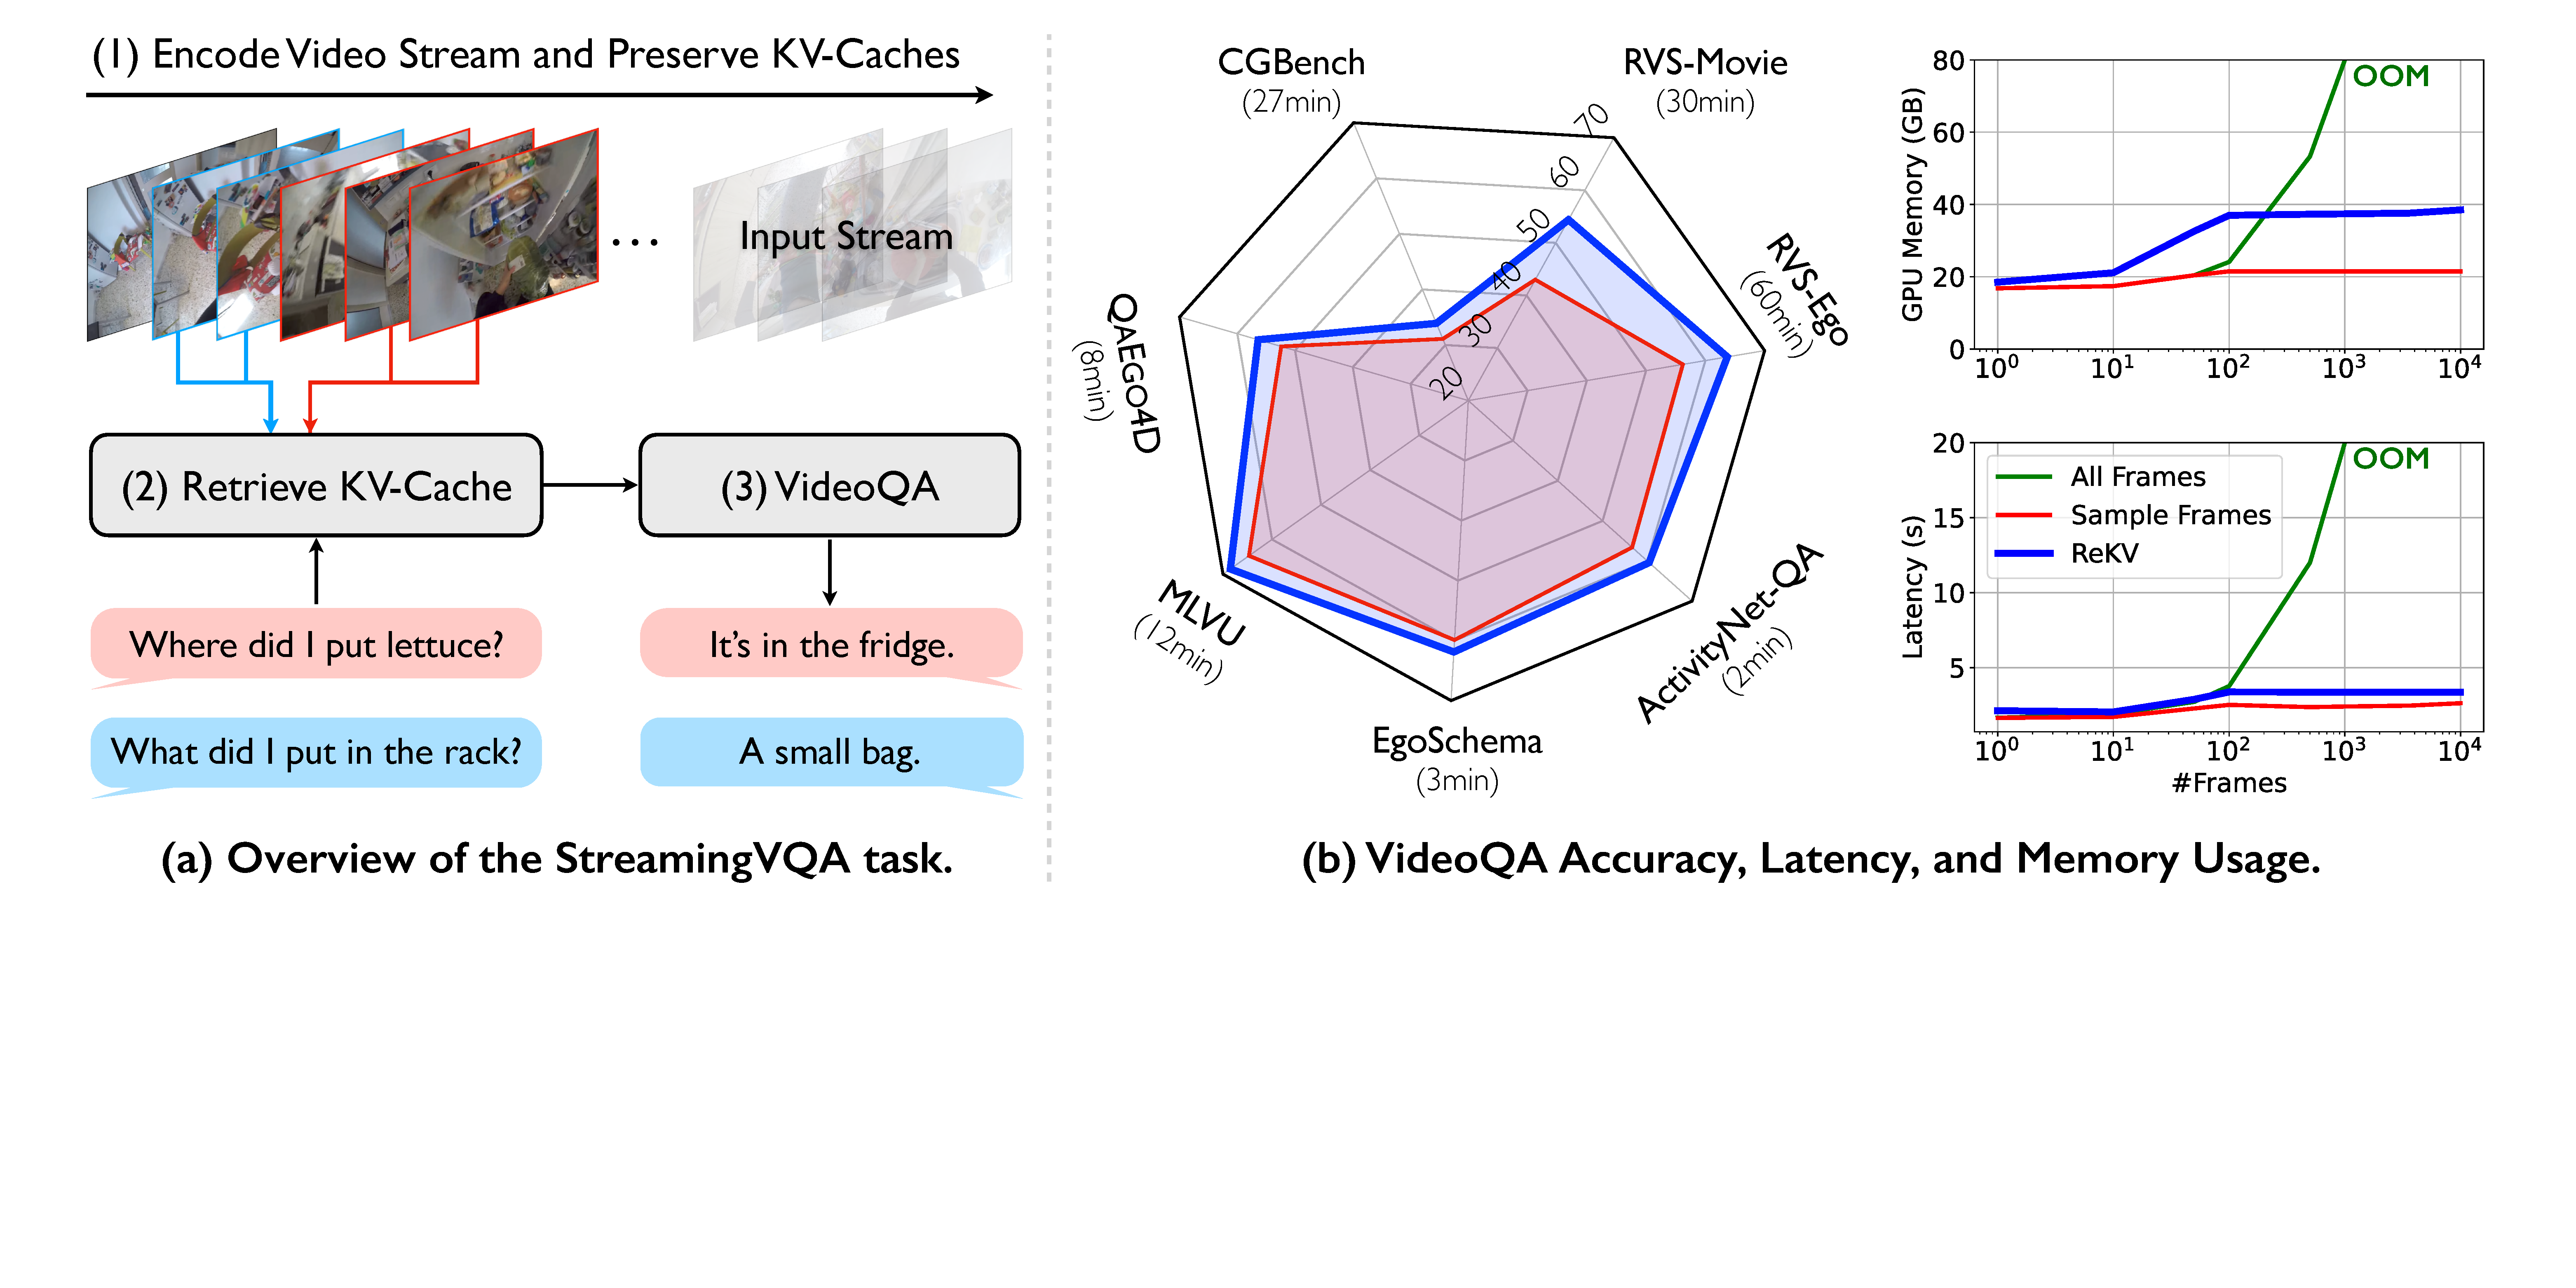
\includegraphics[height=\myfigheight, trim={365pt 0 251pt 0}, clip]{figures/teaser.pdf}}}
        \centering
        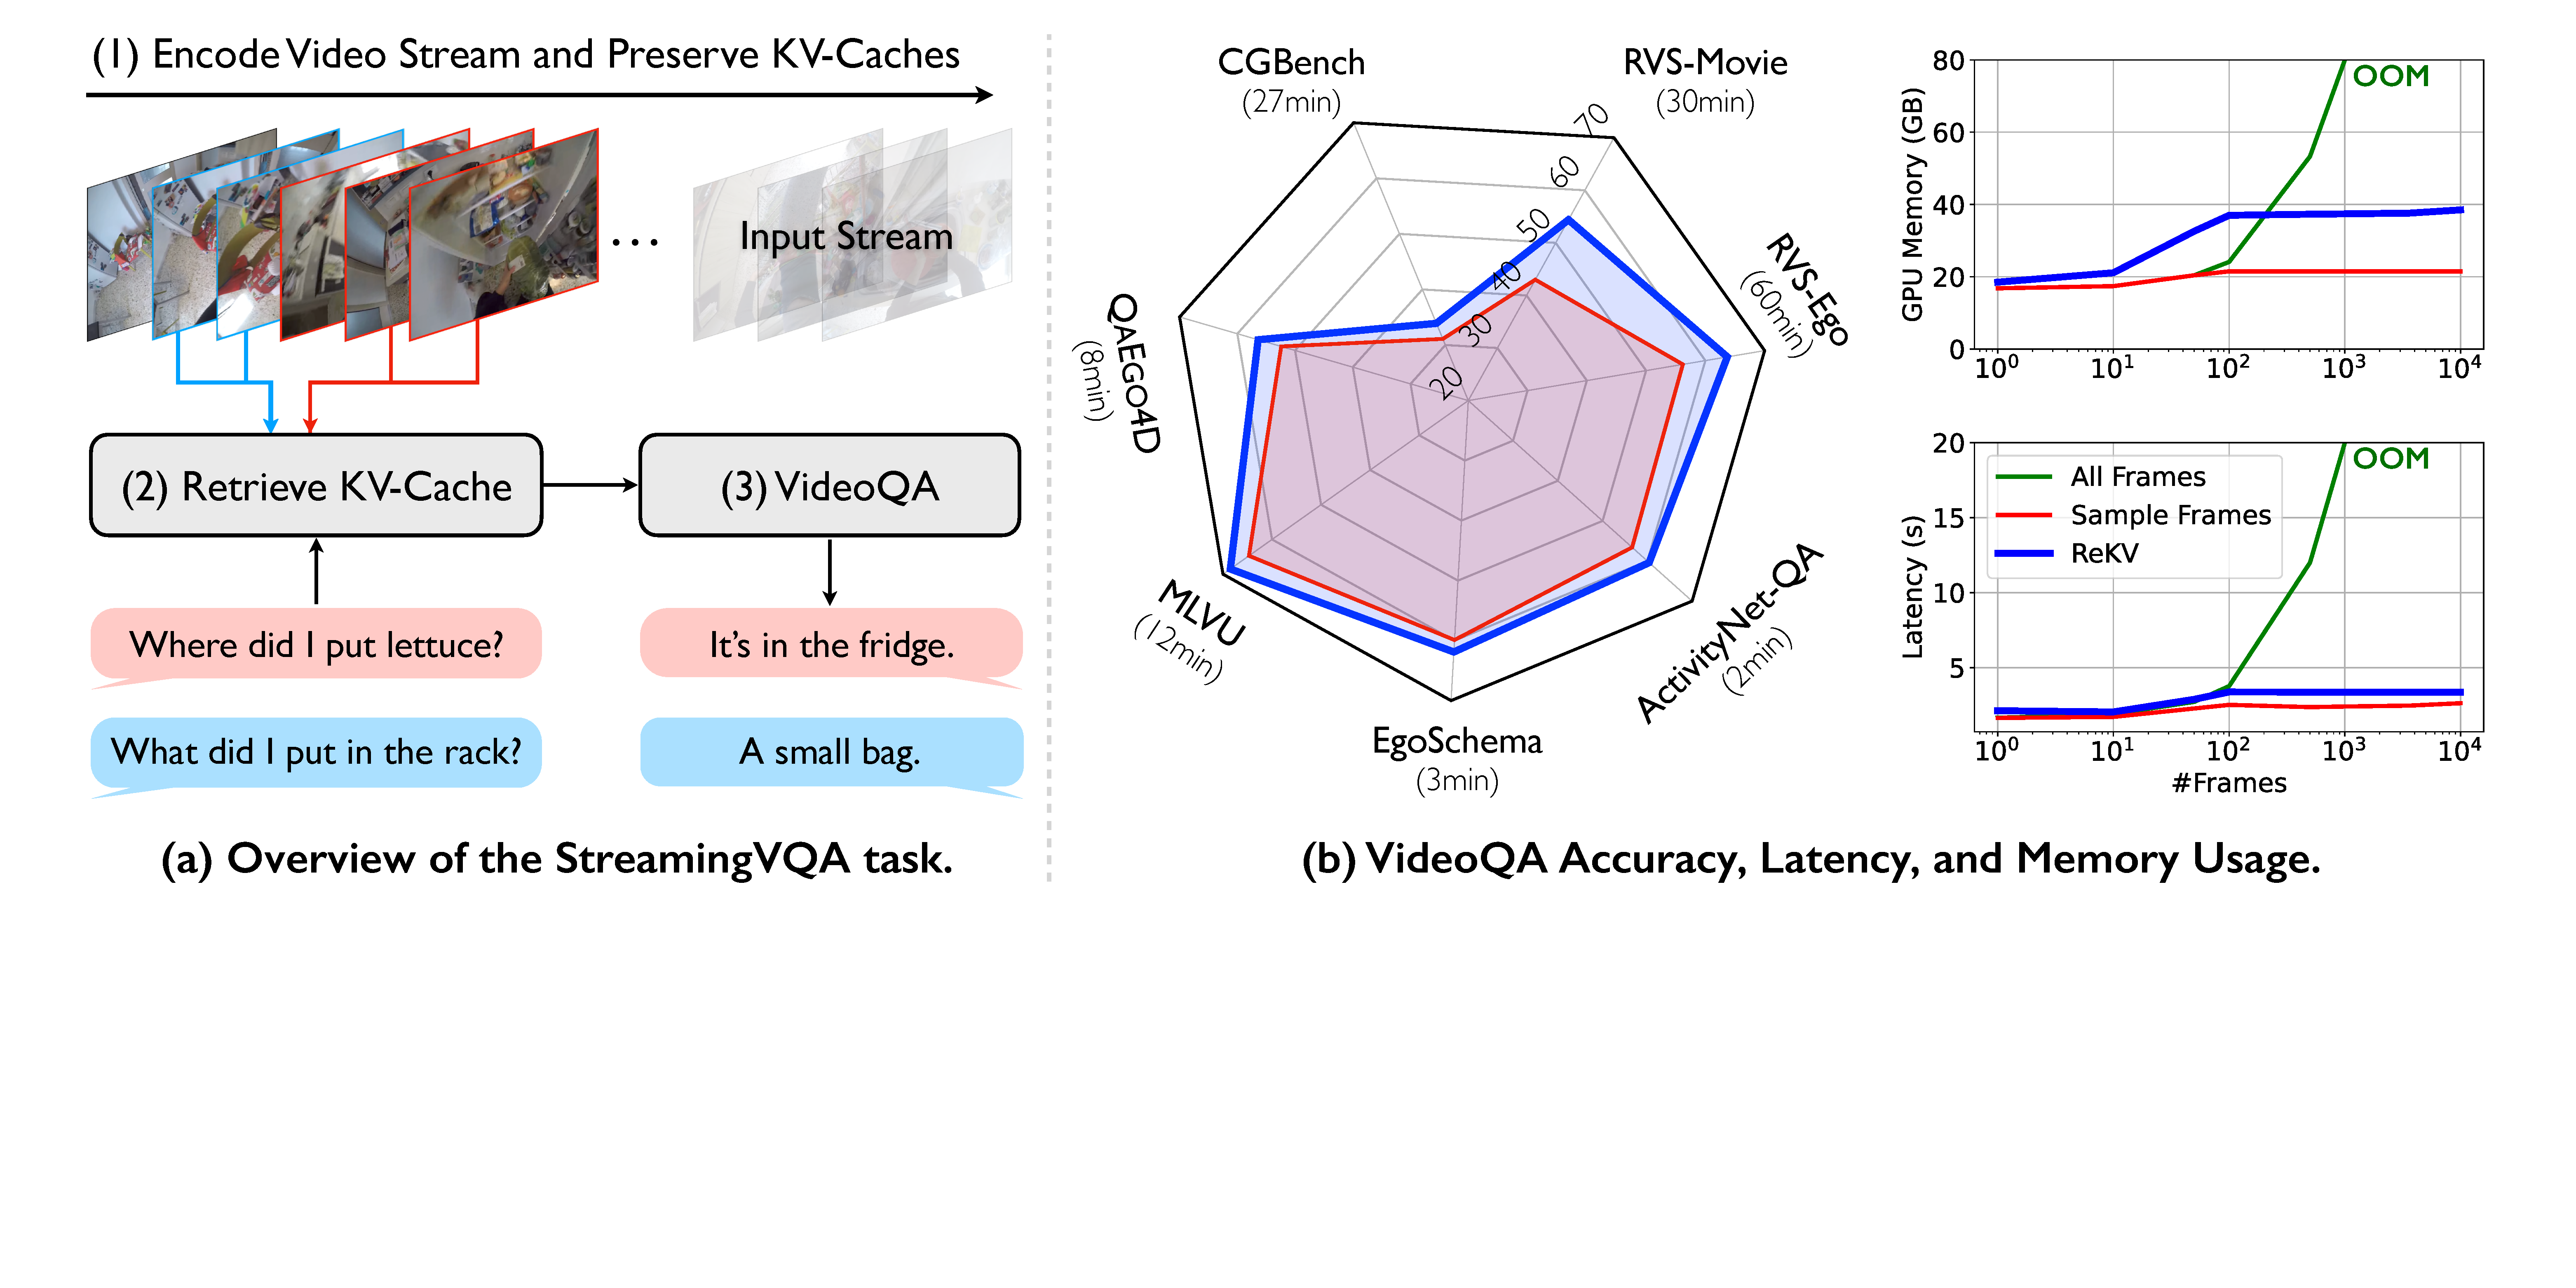
\includegraphics[height=\myfigheight, trim={365pt 0 251pt 0}, clip]{figures/teaser.pdf}
        \caption{Attention Analysis}
        \label{fig:teaser_b}
    \end{subfigure}
    % --- 子图 (c) ---
    \begin{subfigure}{\widthof{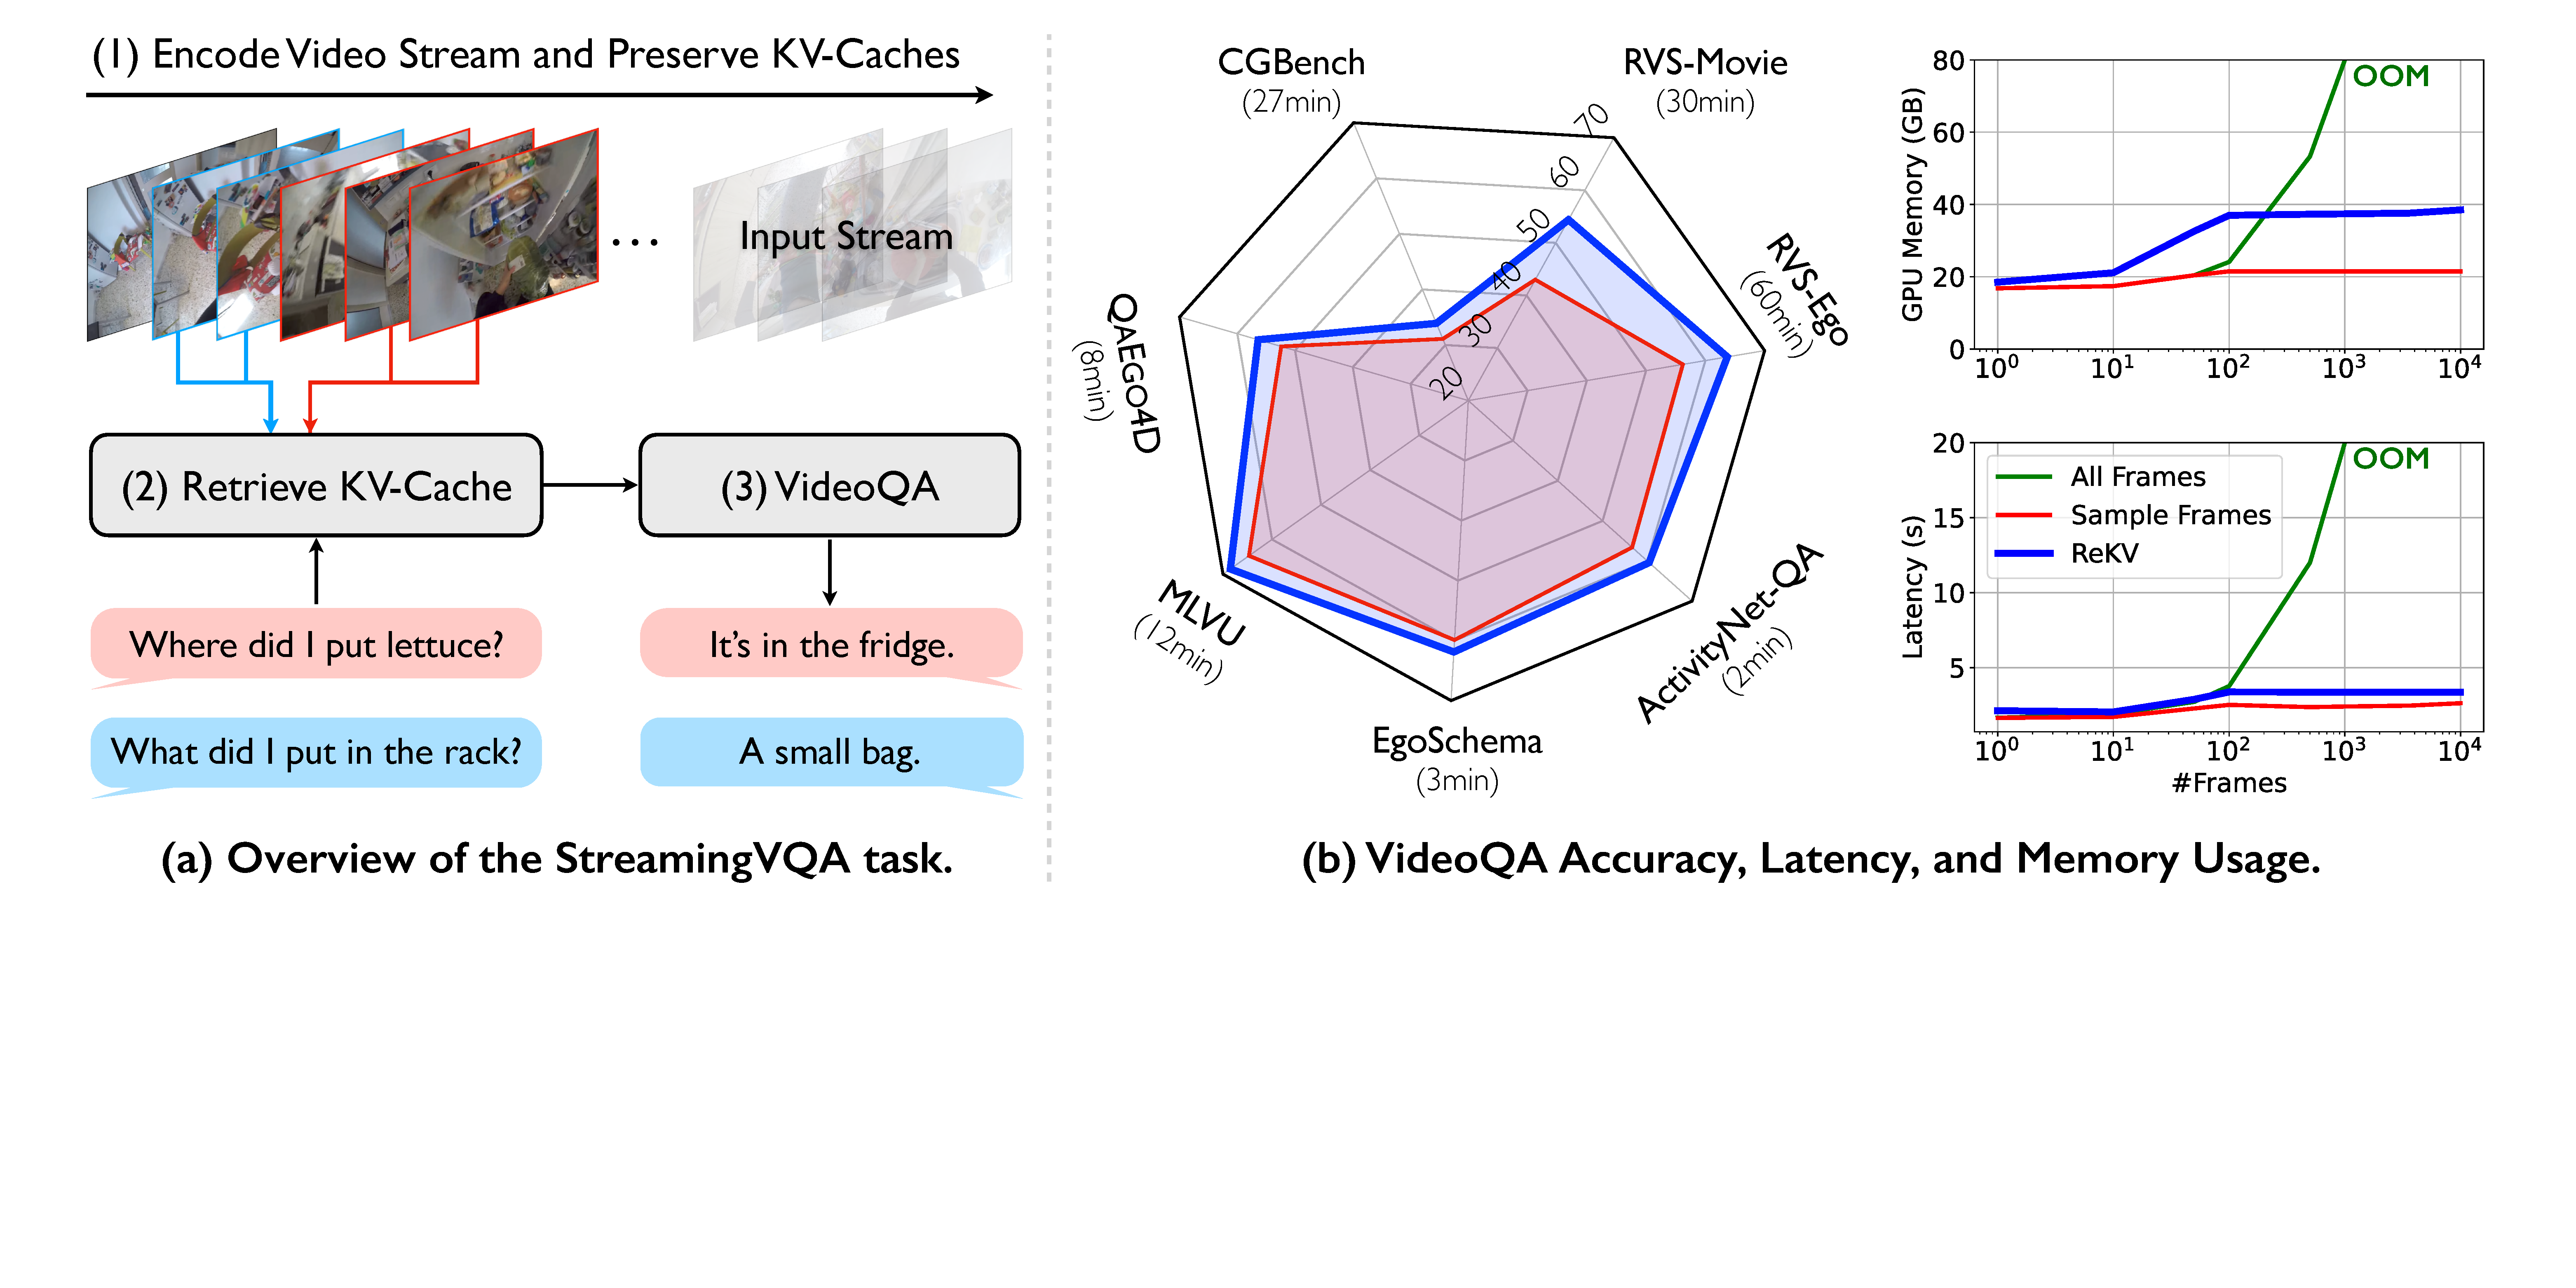
\includegraphics[height=\myfigheight, trim={529pt 0 0 0}, clip]{figures/teaser.pdf}}}
        \centering
        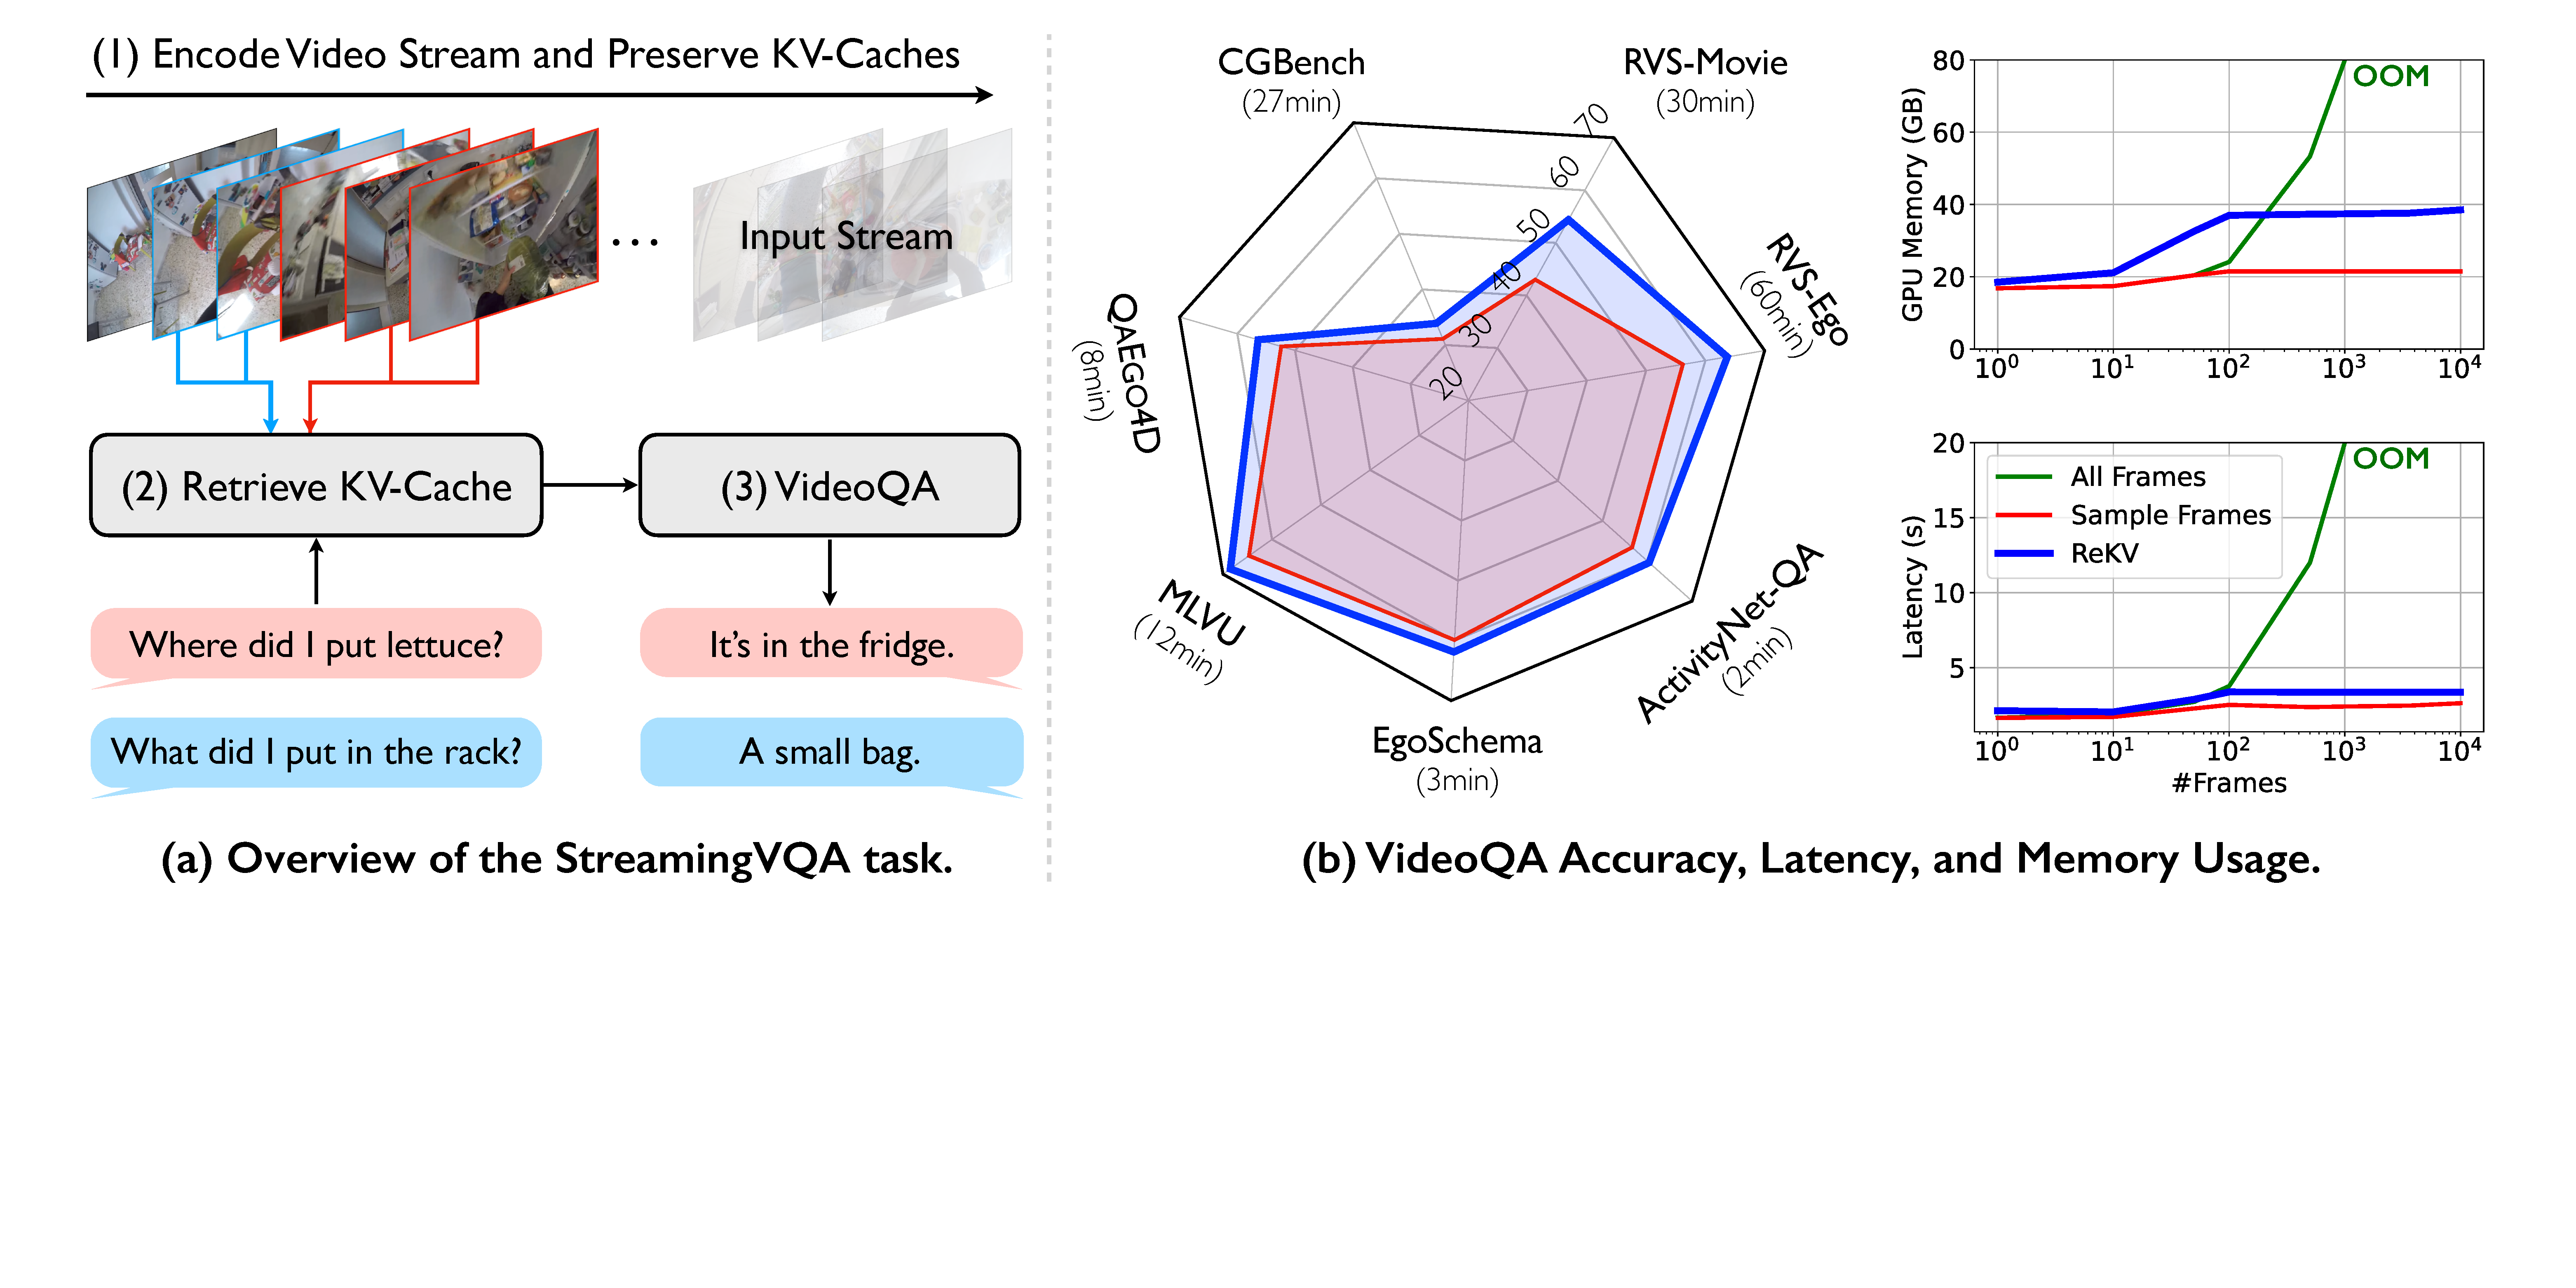
\includegraphics[height=\myfigheight, trim={529pt 0 0 0}, clip]{figures/teaser.pdf}
        \caption{Efficiency Test}
        \label{fig:teaser_c}
    \end{subfigure}
    \caption{\textbf{Left}: \hermes is a training-free approach for efficient streaming video understanding, enabling stable inference by reusing KV cache and performing hierarchical management of video tokens stored in KV cache. \textbf{Middle}: \hermes is based on a mechanistic investigation of the layer-wise attention preferences over hierarchical video information. \textbf{Right}: We evaluate \llava on a single A800 GPU (80 GB). As input frames increase, \hermes consistently maintains extremely low latency (TTFT < 30 ms) and stable GPU memory consumption, exhibiting no risk of OOM errors and requiring no auxiliary external computational resources.}
\end{figure*}



\section{Introduction}
\label{sec:introduction}

% 必须强调流式视频推理的三个重点:1. 稳定准确的推理性能(accuracy) 2. 实时响应 3. 方便端侧设备部署的低GPU memory usage

% 流式输入带来的新挑战

Recent years have witnessed remarkable evolution in the capabilities of Multimodal Large Language Models (MLLMs) in video understanding tasks~\cite{gemini25, li2024llavaonevisioneasyvisualtask, bai2025qwen3vltechnicalreport}.
% Specifically, these models have demonstrated comprehensive understanding and reasoning abilities across various temporal durations and diverse downstream tasks~\cite{li2024mvbenchcomprehensivemultimodalvideo, fu2025videommefirstevercomprehensiveevaluation, mangalam2023egoschemadiagnosticbenchmarklongform}.
Despite the progress, the rapid emergence of real-time applications demands stable long video understanding, low-latency response, and memory-efficient deployment. 
%Consequently, the research frontier is shifting from offline paradigms to streaming video understanding.
%has imposed rigorous demands on MLLMs regarding long temporal context understanding, low-latency inference, and memory efficiency. Consequently, the research frontier is shifting from traditional offline inference paradigms toward streaming inference capable of processing continuous video inputs.
% 现有的offline compression方法由于流式输入的特殊性,无法直接使用
However, existing MLLMs struggle to simultaneously satisfy these requirements on streaming videos.
% Some works streaming methods necessitate expensive model-specific training~\cite{wang2025streambridgeturningofflinevideo, xu2025streamingvlmrealtimeunderstandinginfinite, zeng2025streamforestefficientonlinevideo}, leaving training-free approaches relatively underexplored.
Notably, TimeChat-Online~\cite{timechatonline} observes that a large number of streaming video tokens are redundant, motivating compression methods to address these challenges. While numerous compression techniques have been proposed for offline videos~\cite{wang2025videotreeadaptivetreebasedvideo, yang2024visionziplongerbetternecessary, tao2025dycokedynamiccompressiontokens}, most are ill-suited for memory management in streaming scenarios, as streaming inputs are unpredictable in future frames and queries.
%posing significant challenges for prior static compression methods.
% 现有流式压缩方法的局限,主要有两点: 1. 依赖外挂式记忆和临时检索,时延高。内置式记忆探索得较少,将记忆能力内化入模型很重要 2. 很多是模型特定的训练方法,开销大,不够通用(相对training-free)

To adapt to streaming inputs, recent research introduces specialized memory management techniques, which generally fall into two paradigms: external memory and internal memory. External memory methods store video content as captions or raw vision patches in databases, and perform ad-hoc retrieval and multimodal prefilling at query time~\cite{xiong2025streamingvideounderstandingmultiround, yang2025streamagentanticipatoryagentsstreaming}, suffering from high latency and a lack of end-to-end cohesion. Additionally, many of these methods necessitate costly model-specific training~\cite{wang2025streambridgeturningofflinevideo, xu2025streamingvlmrealtimeunderstandinginfinite, zeng2025streamforestefficientonlinevideo}. In contrast, internalizing memory directly into the key-value cache (KV cache) remains underexplored, yet is crucial for low-latency responses and seamless end-to-end reasoning over stored video contexts. Moreover, KV cache naturally acts as a latent, model-intrinsic memory~\cite{hu2025memoryageaiagents} that frequently interacts with the video stream, making it particularly suitable for training-free memory management. ReKV~\cite{di2025streamingvideoquestionansweringincontext} and LiveVLM~\cite{ning2025livevlmefficientonlinevideo} are representative training-free, cache-based methods for streaming memory management. They store previous video segments in external CPU or disk and need to perform an additional retrieval when a user query arrives, which still rely on external computational resources and leads to significant latency. StreamMem~\cite{yang2025streammemqueryagnostickvcache} leverages chat template tokens to guide compression but lacks fine-grained KV management and mechanistic interpretability.%\jlfu{Discussing how our method differs from other KV-cache–based approaches (e.g., ReKV, StreamMem, and LiveVLM)}

% 正式介绍HERMES这个方法,顺带再提一个之前工作的不足:缺乏机制可解释性

To overcome the aforementioned limitations of existing streaming video methods, we propose \hermes (KV Cache as \underline{\textbf{H}}i\underline{\textbf{ER}}archical \underline{\textbf{M}}emory for \underline{\textbf{E}}fficient \underline{\textbf{S}}treaming Video Understanding), a training-free and plug-and-play approach that can be seamlessly integrated into existing MLLMs. %as shown in \cref{fig:teaser}. 
Grounded in a mechanistic investigation of layer-wise attention shown in~\cref{fig:teaser_b}, we conceptualize KV cache as a hierarchical memory framework that stores video information across multiple levels of granularity: 
%shallow layers as sensory memory, deep layers as long-term memory and middle layers as transitional working memory.
shallow layers function as sensory memory, exhibiting a strong recency bias toward newly arriving frames; deep layers act as long-term memory, focusing on frame-level rhythmic anchor tokens; and middle layers serve as transitional working memory that balances recency information with frame-level semantic representations.
Our method \hermes comprises three components: \emph{hierarchical KV cache management}, \emph{cross-layer memory smoothing}, and \emph{position re-indexing}. During inference, \hermes reuses the compact KV cache and requires no auxiliary computations or external devices upon the arrival of user queries, thereby guaranteeing real-time responses. Experiments show that \hermes maintains stable and accurate performance with up to 68\% fewer video tokens, while maintaining consistently low response latency and a constant GPU memory footprint.

% In contrast to many prior multimodal compression works that rely on heuristic techniques~\cite{kim2025infinipotvmemoryconstrainedkvcache, yang2025streammemqueryagnostickvcache, chen2025streamkvstreamingvideoquestionanswering}, which struggle with limited interpretability and reliability, our approach is based on a mechanistic investigation of layer-wise attention preference for hierarchical video information.

%Grounded in a mechanistic investigation of layer-wise attention preferences for hierarchical video tokens, we conceptualize the key-value cache (KV cache) as a hierarchical memory framework that stores video information across multiple levels of temporal granularity.

% We observe that the shallow, middle, and deep decoder layers of MLLMs correspond to the short-term, mid-term, and long-term memory of streaming video information, respectively.


% \begin{itemize} [leftmargin=*]
% \itemsep0em 
% \item 
% \textbf{Shallow Layers as Short-term Memory}: For the short-term video memory stored in the shallow layers, where attention exhibits a strong preference for temporally recent video tokens, we employ a First-In-First-Out (FIFO) eviction strategy to only keep the recent video tokens.
% \item
% \textbf{Middle Layers as Mid-term Memory}: The middle layers serve as a transition from short-term to long-term memory. These layers increasingly focus on video content that is temporally distant from the time point of user queries, with attention patterns becoming progressively sparser. Token eviction in this stage is determined by a weighted combination of attention and recency scores of video tokens. To account for unpredictable user queries, we utilize specifically designed local and global guidance prompts to steer the compression.
% \item
% \textbf{Deep Layers as Long-term Memory}: In the deep layers, attention is extremely sparse, and the bias toward recent video tokens largely disappears. These layers primarily capture global and abstract semantic information. Compression is guided by attention scores from the global guidance prompt. To maximize the preservation of video information, evicted tokens are aggregated into a summary token maintained at the end of the sequence.
% \end{itemize}

%Beyond the hierarchical design, we introduce \emph{layer consistency} as a smoothing mechanism. This allows the long-term memory in deeper layers to provide feedback for token retention in earlier layers, thereby mitigating information inconsistencies across different memory stages. 

% Finally, to support potentially infinite video streams, especially in resource-limited scenarios, we maintain a fixed and compact GPU memory footprint at all times. We implement a \emph{soft position encoding reassignment} method to ensure both stable comprehension performance and an enhanced perception of recent temporal dynamics, which are essential for streaming understanding~\cite{xu2025streamingvlmrealtimeunderstandinginfinite}.


To summarize, our main contributions are as follows:
\begin{enumerate}[leftmargin=*]
\itemsep0em 
\item
Grounded in a mechanistic analysis on attention visualization, we pioneer the conceptualization of KV cache as a hierarchical video memory framework across multiple granularities.

\item
We propose \hermes, a training-free method for streaming video understanding by reusing hierarchically managed KV cache. Despite reducing video tokens by up to 68\%, \hermes achieves competitive accuracy, with gains of up to 11.4\% on streaming benchmarks.

\item
\hermes exhibits outstanding efficiency in streaming scenarios. Compared to the prior training-free SOTA method, it achieves up to a 10$\times$ speedup in latency. With a constant, compact GPU memory footprint and no auxiliary computation at query time, \hermes ensures consistently low-latency responses.

\end{enumerate}